% !TEX root = /media/ueslei/Ueslei/INPE/PCI/Guia_COAWST/main.tex
\chapterimage{ocean2.jpg}
\chapter{Construindo o SWAN}

\noindent O SWAN utiliza o arquivo \textit{SWAN.EDT} para ler os  arquivos de grade (\textit{swan\_coord.grd}) e
          de batimetria (\textit{swan\_bathy.bot}). Também é possivel definir uma grade numérica dentro do próprio
          \textit{SWAN.EDT} e indicar o arquivo de batimetria que será lido e associado com a grade definida.
\bigskip

\noindent Como exemplo, serão criados os arquivos do SWAN a partir da grade do ROMS, porém sem a introdução de dados iniciais, 
          pois a implementação de uma grade dentro do \textit{SWAN.EDT} não é trivial    
\bigskip

\noindent Para as condições de fronteiras do SWAN, os campos de vento serão provenientes do WRF, via acoplamento, logo
          as ondas geradas estão associados aos sistemas atmosféricos representados nestas simulações. Sem as informações 
          de contorno, as ondas simuladas serão geradas apenas dentro do límite do domínio, desconsiderando a energia que 
          está saindo ou entrando na grade.
\bigskip

\noindent Utilizaremos o script do MATLAB, \textit{make\_swan.m}, para gerar os arquivos. O script está localizado em:  
\bigskip

\begin{bashcode}
/home/nome.sobrenome/repositorio/SWAN_scripts
\end{bashcode}
\bigskip

\noindent Conforme a Figura \textcolor{bleu_cite}{\ref{makeswan}}, o script possui a seguinte construção:
\bigskip

\begin{figure}[H]
    \centering
    \captionsetup{justification=centering}
    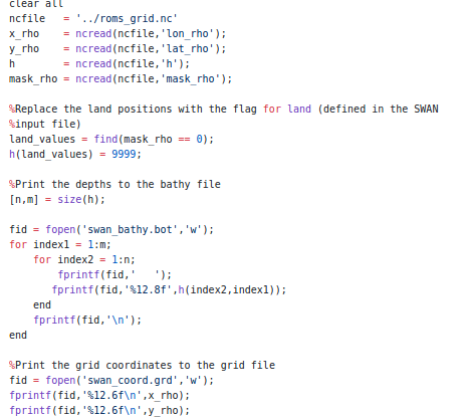
\includegraphics[width=0.47\textwidth]{makeswan.png}
    \caption{O script \textit{make\_swan.m}.}
    \label{makeswan}
\end{figure}
\bigskip

\noindent Para gerar os dois arquivos do SWAN, procure no script a variável \textit{ncfile} e altere o diretório 
          para o caminho onde está sua grade do ROMS.
\bigskip

\noindent Execute o script e serão criados os dois arquivos: \textit {swan\_coord.grd} e \textit{swan\_bathy.bot}. 
           Os dois arquivos deverão ser colocados dentro da sua pasta de projetos.
\bigskip

\chapter{Construindo o Budgell's Sea Ice Model}
\bigskip

\noindent O modelo de gelo marinho está integralmente acoplado ao ROMS, de modo que, após gerada as condições do 
          ROMS com os dados de gelo (Veja a Seção \textcolor{bleu_cite}{\ref{model2romssec}}), para ativar o modelo 
          de gelo marinho basta modificar o arquivo \textit{.h} do ROMS no seu projeto e acrescentar as seguintes 
          opções (Figura \textcolor{bleu_cite}{\ref{hiceroms}}):
\bigskip

\begin{itemize}
    \item \textbf{ICE\_MODEL}: Define o modelo de gelo marinho;
    \item \textbf{ANA\_ICE}: Define condições iniciais analíticas para o gelo marinho 
    \item \textbf{ICE\_THERMO}: Define a termodinâmica do gelo;  
    \item \textbf{ICE\_MK}: Define a termodinâmica de gelo proposta por \textcite{Mellor1989}. Atualmente é a única opção disponível;
    \item \textbf{ICE\_MOMENTUM}: Define a componente de \textit{momentum} do gelo;
    \item \textbf{ICE\_MOM\_BULK}: Defina para computar o estresse entre água e gelo;
    \item \textbf{ICE\_EVP}: Define a reologia proposta por \textcite{Hunke1997} e \textcite{Hunke2001};
    \item \textbf{ICE\_STRENGTH\_QUAD}: Defina para ativar a força quadrática do gelo proposta por \textcite{Overland1988};
    \item \textbf{ICE\_ADVECT}: Defina para ativar a advecão dos traçadores do gelo.
    \item \textbf{ICE\_SMOLAR}: Defina para usar \textit{MPDATA} como traçador do gelo. Atualmente é a única opção disponível;   
    \item \textbf{ICE\_UPWIND}: Defina para adveção do vento;
    \item \textbf{ICE\_BULK\_FLUXES}: Defina para computar a parametrização de fluxos de calor Bulk para o gelo;
    \item \textbf{ICE\_DIAGS}: Define o diagnóstico do gelo marinho.
\end{itemize}
\bigskip

\begin{figure}[H]
    \centering
    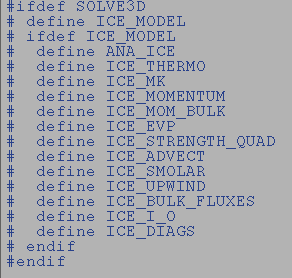
\includegraphics[width=0.3\textwidth]{hiceroms.png}
    \caption{Captura de tela do arquivo \textit{.h} do ROMS.}
    \label{hiceroms}
\end{figure}
\bigskip

\noindent Para ter mais informações sobre o modelo, recomenda-se a leitura de \textcite{hedstrom2018}.
\bigskip

\noindent Obtenha o arquivo \textit{.in} para o modelo de gelo marinho. Copie o arquivo \textit{ice.in} dentro do 
          repositório do Kerana e adicione ao seu projeto.
\bigskip

\begin{bashcode}
    /home/nome.sobrenome/repositorio/ICE_scripts
\end{bashcode}
\bigskip
    
\noindent Modifique o arquivo \textit{.in} do ROMS, apontando o diretório do arquivo \textit{ice.in} do 
          modelo de gelo marinho. Procure pela variável \textit{IPARNAM} e adicione o diretório:
\bigskip

\begin{bashcode}
nedit ocean.in
IPARNAM =  ice.in
\end{bashcode}

